\section{Paketstruktur}
\textcolor{blue}{\textit{Dieser Abschnitt beschreibt im Wesentlichen eine grobe Zerlegung der zu entwickelnden Anwendung in Pakete und deren Zusammenhänge. Dabei sollen Zusammenhänge und Abhängigkeiten zwischen den Paketen beschrieben werden.\\\\
Die hier definierten Pakete sind logische Einheiten oder gemeinsam genutzte Einheiten, die aus beliebig vielen Klassen bestehen können, welche gemeinsam die Funktionalität durch das Paket zusammenfassen. Die Aufteilung von Klassen zu Paketen muss sich dabei nicht an den strukturellen Eigenschaften der Architektur (z.B. Komponenten) orientieren. Vielmehr soll die Zerlegung in Pakete der besseren Strukturierung, Organisation, Arbeitsteilung bei Implementierung und Übersichtlichkeit der in der gesamten Architektur verwendeten Klassen dienen.\\\\
Das folgende Paketdiagramm führt Pakete ein und beschreibt ihre Abhängigkeiten. 
}}

\begin{figure}[H]
\centering
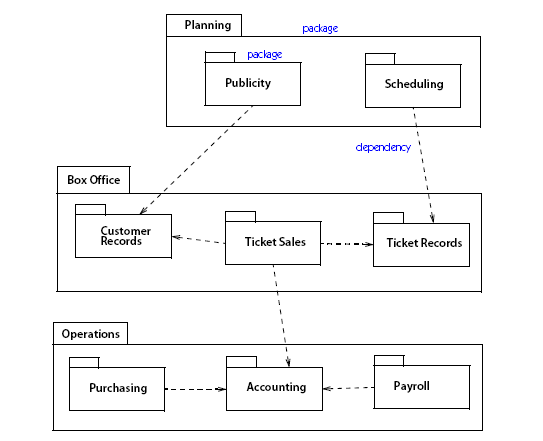
\includegraphics[width=0.8\textwidth]{img/Paketstruktur.png}
\caption{\textcolor{blue}{Durch eigene Diagramme ersetzen}}
\label{Paketstruktur}
\end{figure}
